%%%%%%%%%%%%%%%%%%%%%%%%%%%%%%%%%%%%%%%%%%%%%%
%       Plantilla Informes Isaias Cardenas
%%%%%%%%%%%%%%%%%%%%%%%%%%%%%%%%%%%%%%%%%%%%%%

\documentclass[letterpaper,12pt]{report}
\usepackage[right=2cm,left=3cm,top=2cm,bottom=2cm,footskip=1.4cm]{geometry}%margenes de la pagina

\usepackage{ucs}
\usepackage[utf8x]{inputenc}
\usepackage[spanish, es-tabla]{babel}
\usepackage[T1]{fontenc}
\usepackage{blindtext}
\usepackage{enumitem}
\usepackage{graphicx}
\usepackage{listings} % escribir codigo
\usepackage{algpseudocode} % escribir algoritmos
\graphicspath{ {./images/} }
\usepackage{multicol} % multicolumnas
% \usepackage{subfigure} % incluir multiples imágenes en una figura
\usepackage{float} % poscicionar imagenes
% \fontfamily{ppl}\selectfont % change font

% \RequirePackage{hyperref}
% \RequirePackage{url} %citacion de URL
% \usepackage{hyperref}
\linespread{1.5} %interlineado

%borra la palabra "capitulo"
\usepackage{titlesec}
\titleformat{\chapter}[display]
    {\normalfont\huge\bfseries}{}{0pt}{\Huge}
\titlespacing*{\chapter}
    {0pt}{10pt}{40pt}


\begin{document}
\renewcommand{\contentsname}{Tabla de Contenido}
\begin{titlepage}
\begin{center}
UNIVERSIDAD DE SANTIAGO DE CHILE\\
FACULTAD DE INGENIERÍA\\
DEPARTAMENTO DE INGENIERÍA INFORMÁTICA\\
\begin{figure}[htb]
\begin{center}

\includegraphics[width=4.5cm]{logo.png}
\end{center}
\end{figure}

\vspace*{0.7in}
\begin{Large}
\textbf{Manual de usuario: Buscaminas} \\
\end{Large}
\vspace*{0.3in}

\vspace*{2in}

\end{center}
\begin{flushright}

\begin{tabular}{lll}
Alumno & : & Isaías Cárdenas\\
Rut & : & 18750177-6\\
Profesor & : & Pablo Schwarzenberg\\
Curso & : & Laboratorio estructuras de datos y análisis de algoritmos\\
Ayudantes & : & Sebastián Vallejos\\
          &  & Javiera Torres\\
Fecha de entrega & : & 30 de agosto de 2017
\end{tabular}
\end{flushright}
\end{titlepage}

\tableofcontents
% \listoffigures
% \listoftables

\chapter {Introducci\'on}

\section {Introducci\'on}

El presente documento hace referencia al uso del proyecto ``Buscaminas'', el cual es la primera entrega para el laboratorio de la asignatura Estructuras de datos y análisis de algoritmos. El uso adecuado de un programa es escencial para su correcto funcionamiento y es por esta razón que es indispensable que el usuario lea detenidamente el manual de usuario a modo de minimizar los errores de uso y, en caso de que el programa presente errores, éstos sean detectados con alta seguridad de que el problema reside en el código y no en su uso incorrecto por parte del usuario. A continuación se detallan las entradas de usuario válidas y las salidas que el programa entrega, la simbología utilizada para representar la interfáz gráfica y sus respectivos significados y los posibles errores que podrían provocar el uso incorrecto de el programa por parte del usuario.

\chapter {C\'omo compilar y ejecutar}

\section {Directorios y archivos}

En total el proyecto consta de cuatro archivos principales contenidos en el directorio ``/src'' cada uno de ellos con sus archivos headers correspondientes(archivos con extensión .h), se detallan los contenidos a continuación: 

\begin{description}[align=left]

\item [BoardBlock.c:] 
    En este archivo se define la estructura BoardBlock que será utilizada como la representación de las casillas del tablero y la definición de la función que inicializará a esta estructura. 

\item [Board.c:]
    Board.c contiene la definición de la estructura Board que generará el tablero de juego a partir de la estructura anterior, además contiene las definiciones de las funciones que interactuan con ésta estructura.

\item [functions.c:]
    Aqui se definen las funciones auxiliares para la jugabilidad principal, estas estructuras no tienen interacción directa con las estructuras mencionadas anteriormente, es por ello que se especifican en un archivo aparte.

\item [Buscaminas.c:]
    El contenido de este fichero es la jugabilidad del buscaminas como tal, se realiza la interacción entre las estructuras Board y BoardBlock ademas de las funciones auxiliares. Se maneja la interacción entre el usuario y el programa mediante una pseudo-interfaz y se controla el flujo de la jugabilidad. La funcionalidad del programa se engloba en una función principal llamada ``run''.

\end{description}

\section {Entorno Linux}

Además de los archivos mencionados se crea el archivo ``main.c'' ubicado en el directorio raíz del proyecto, como su nombre lo dice este archivo contiene la función main que hace posible la ejecución del programa. Para compilar el programa es necesario ubicarse en el directorio del proyecto via consola y desde ahí ejecutar el siguiente comando: 

\begin{lstlisting}[language=bash]
gcc main.c src/Buscaminas.c src/Board.c src/BoardBlock.c src/functions.c
\end{lstlisting}

El proyecto es compilado a través de ``gcc'' (GNU Compiler Collection) y generará un archivo ejecutable llamado ``a.out'' en el directorio del proyecto. La figura \ref{fig:gccLinux} ejemplifica lo anterior en la terminal de un sistema operativo Linux:

\begin{figure}[H]
    \centering
    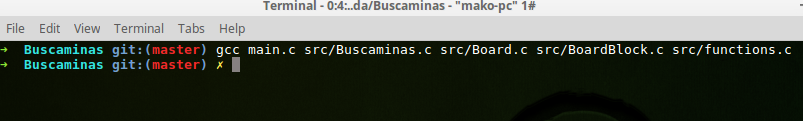
\includegraphics[width=1\textwidth]{gccLinux.png}
    \caption{Compilación del proyecto en entorno Linux}
    \label{fig:gccLinux}
\end{figure}

Para ejecutar el archivo generado bastará con realizar el siguiente comando en la terminal:

\begin{lstlisting}[language=bash]
./a.out
\end{lstlisting}

La figura \ref{fig:ejecLinux} muestra la ejecución del archivo generado en el directorio una vez compilado el proyecto en un sistema operativo Linux.

\begin{figure}[H]
    \centering
    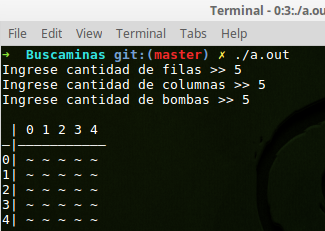
\includegraphics[width=0.6\textwidth]{ejecLinux.png}
    \caption{Ejecución del proyecto en entorno Linux}
    \label{fig:ejecLinux}
\end{figure}

Si el usuario lo desea puede cambiar el nombre del archivo ejecutable mediante la opción ``-o <nombreArchivo>'', de este modo el ejecutable a.out pasará a ser <nombreArchivo> y puede ser compilado del mismo modo.

\section {Entorno Windows}

Para compilar la aplicación en un sistema operativo Windows es necesario tener instalado un compilador para el lenguaje C, esto puede ser realizado mediante MinGW (Minimalist GNU for Windows). Dicho esto el proceso de compilación es el mismo que en un entorno linux mediante ``gcc''. La figura \ref{fig:gccWin} muestra la compilación del programa en un sistema operativo mediante gcc:

\begin{figure}[H]
    \centering
    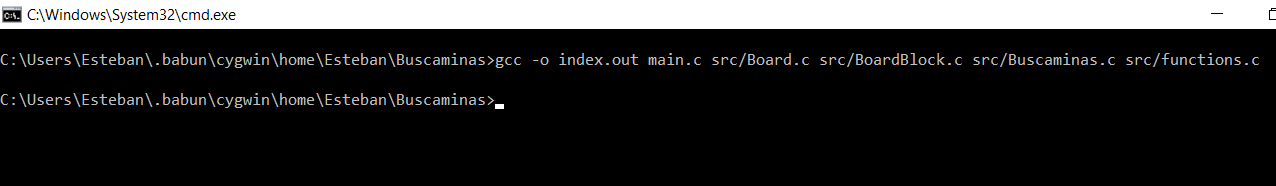
\includegraphics[width=1\textwidth]{gccWin.png}
    \caption{Compilación del proyecto en entorno Windows}
    \label{fig:gccWin}
\end{figure}

Luego de compilar el programa se generará el archivo ejecutable, que en este caso fue nombrado ``index.out'', que puede ser ejecutado de la misma manera que en un sistema operativo Linux, tal y como lo muestra la figura \ref{fig:ejecWin} a continuación:

\begin{figure}[H]
    \centering
    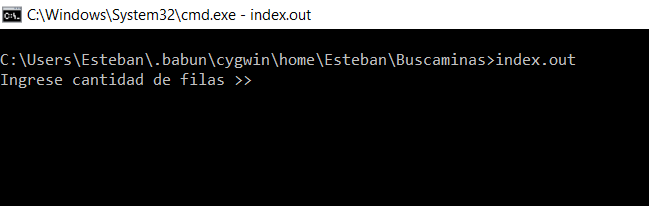
\includegraphics[width=0.8\textwidth]{ejecWin.png}
    \caption{Ejecución del proyecto en entorno Windows}
    \label{fig:ejecWin}
\end{figure}

\chapter{Funcionalidades del programa}

Una vez ejecutado el programa se le pedirá al usuario que ingrese la cantidad de filas, columnas y bombas que tendrá el tablero de juego, estos valores deben ser números enteros naturales para que el programa funcione correctamente. La cantidad de filas y columnas no deben ser mayores a 100 y la cantidad de bombas deben ser menor al área del tablero menos 2 casillas, de este modo el usuario no perderá en la primera jugada ni ganará en la primera jugada.

Luego de ingresar los valores se generará el tablero de juego con los siguientes símbolos:

\begin{description}[align=left]

\item [`` \_~ ''] 
    En este archivo se define la estructura BoardBlock que será utilizada como la representación de las casillas del tablero y la definición de la función que inicializará a esta estructura. 

\item [`` ' '':]
    Board.c contiene la definición de la estructura Board que generará el tablero de juego a partir de la estructura anterior, además contiene las definiciones de las funciones que interactuan con ésta estructura.

\item [`` * '':]
    Aqui se definen las funciones auxiliares para la jugabilidad principal, estas estructuras no tienen interacción directa con las estructuras mencionadas anteriormente, es por ello que se especifican en un archivo aparte.

\item [número:]
    El contenido de este fichero es la jugabilidad del buscaminas como tal, se realiza la interacción entre las estructuras Board y BoardBlock ademas de las funciones auxiliares. Se maneja la interacción entre el usuario y el programa mediante una pseudo-interfaz y se controla el flujo de la jugabilidad. La funcionalidad del programa se engloba en una función principal llamada ``run''.

\end{description}

Al iniciar el juego se le pedirá al usuario que ingrese sus jugadas que deben ser ingresadas en el siguiente formato:

\begin{lstlisting}[language=txt]
<< fila columna jugada >>
\end{lstlisting}

En donde ``fila'' y ``columna'' deben ser números naturales menores a 100 y jugada debe ser el carácter ``O'' ó ``X'', para descubirir la casilla o marcar posible bomba respectvamente. El uso incorrecto de las entradas del usuario podrían provocar errores en el funcionamiento del programa.

El usuario podrá descubrir solamente las casillas que no han sido descubiertas y podrá marcar una casilla como posible bomba solamente a aquellas que no hayan sido descubiertas, el uso incorrecto de las acciones del usuario podrían ocasionar un mal funcionamiento del programa. Por otro lado el usuario deberá realizar acciones solo dentro del tablero, si ingresa coordenadas que se encuentran fuera del área del tablero el programa indicará que es una acción incorrecta.

Tras la primera jugada del usuario el programa generará el archivo ``solución.out'' en el que se muestra el contenido del tablero del juego completamente descubierto, es decir, el usuario 

\chapter{Posibles errores}


Se cumplen los objetivos propuestos y los requerimientos solicitados en el plazo estipulado, el uso de punteros y el manejo de memoria dinámica se logra en totalidad logarando crear una matriz bidimencional que contiene estructuras. ...

\end{document}
